\documentclass[SKL-MASTER.tex]{subfiles}
\begin{document}
%=========================================================
\Large
\section*{Training set and testing set}

% This is why datasets are often split into 
%======================================================================== %
%\subsubsection{Training set and testing set}
\begin{itemize}
\item Machine learning is about learning some properties of a data set and applying them to new data. \item This is why a
common practice in machine learning to evaluate an algorithm is to split the data at hand in two sets \textbf{\textit{training data}} and \textbf{\textit{testing data}}.
\end{itemize}

\begin{itemize}
\item We learn data properties and fit the model with the training data, 
\item On the testing set, we test  the mode that we have fitted.
\end{itemize} 

When experimenting with a learning algorithm, it is important not to test the prediction of an estimator on the data used to fit the estimator, as this would not be evaluating the performance of the estimator on new data.
\newpage
\subsection*{KNN (k nearest neighbors) classification example:}

\begin{figure}[h!]
\centering
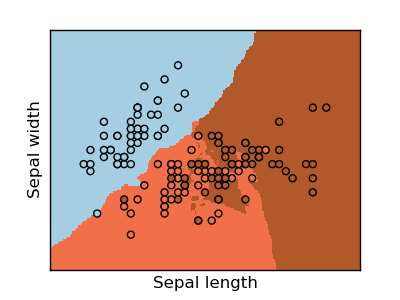
\includegraphics[width=0.5\linewidth]{images/iris_knn1}

\end{figure}

\noindent Firstly, we will split the iris data in training and testing data sets.
We will use a random permutation, to split the data randomly
\begin{framed}
\begin{verbatim}

>>> np.random.seed(0)
>>> indices = np.random.permutation(len(iris_X))
>>> iris_X_train = iris_X[indices[:-10]]
>>> iris_y_train = iris_y[indices[:-10]]
>>> iris_X_test  = iris_X[indices[-10:]]
>>> iris_y_test  = iris_y[indices[-10:]]
\end{verbatim}
\end{framed}
Now we will create and fit a nearest-neighbor classifier
{\large
	\begin{framed}
	\begin{verbatim}
>>> from scikits.learn.neighbors import NeighborsClassifier
>>> knn = NeighborsClassifier()
>>> knn.fit(iris_X_train, iris_y_train)

	NeighborsClassifier(n_neighbors=5, 
	leaf_size=20, algorithm='auto')
\end{verbatim}
\end{framed}
}
Now lets use our model on the test data
\begin{framed}
	\begin{verbatim}
>>> knn.predict(iris_X_test)

	array([1, 2, 1, 0, 0, 0, 2, 1, 2, 0])

>>> iris_y_test

	array([1, 1, 1, 0, 0, 0, 2, 1, 2, 0])
\end{verbatim}
\end{framed}

\end{document}